\documentclass[english]{mlutalk}
% \documentclass[english,handout]{mlutalk}

\title{Overview of T5 and T0\\Grimjack at Touché 2022}
\subtitle{Advanced IR, Winter Semester 2021/22}
\author{Johannes Huck \and Jan Heinrich Reimer}
\institute{Martin Luther University Halle-Wittenberg}
\date{\today}
\titlegraphic{
\includegraphics[width=3cm]{figures/mlu-halle}}

\addbibresource{../literature/literature.bib}

\usepackage{tikz}
\usetikzlibrary{positioning}
\usepackage{listings}
\usepackage{xspace}
\usepackage{biblatex}
\usepackage{tabularx}
\usepackage{booktabs}
\usepackage{graphics,graphicx}

\newcommand{\TF}{\mbox{TF}\xspace}
\newcommand{\TFIDF}{\mbox{TF/IDF}\xspace}
\newcommand{\todocite}{{\smaller\color{red}[CITE]}\xspace}
\newcommand{\todo}[1]{{\smaller\color{red}[#1]}}

\lstset{%
  basicstyle=\ttfamily,
  breaklines=true
}

\begin{document}

\titleframe

\begin{frame}{What is T5?~\cite{RaffelSRLNMZLL2020}}
  \begin{itemize}
    \item Published in: Exploring the Limits of Transfer Learning with a Unified
    Text-to-Text Transformer
    \item Published by Google AI in 2019/2020
    \item Goal: Is it possible to create one architecture to tackle different types of NLP task? 
    \item T5 stands for: \textbf{T}ext-\textbf{t}o-\textbf{T}ext \textbf{T}ransfer \textbf{T}ransformer
  \end{itemize}
\end{frame}


\begin{frame}{Examples of T5 tasks}
  \begin{figure}
      \center
      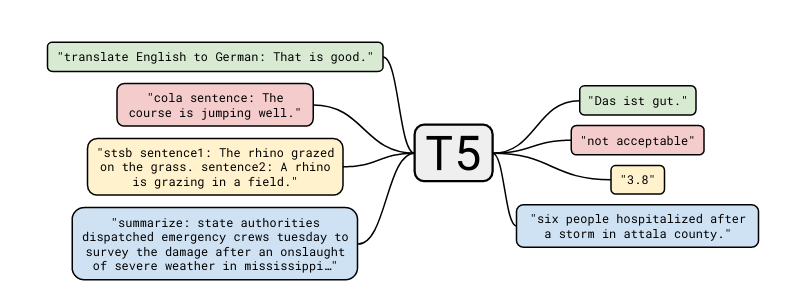
\includegraphics[scale=0.45]{figures/t5-examples.png}
  \end{figure}
\end{frame}

\begin{frame}{Architecture of T5}
    \begin{itemize}
      \item Follows the transformer architecture by Vaswani et. al~\cite{VaswaniSPUJGKP2017}
      \item An input sequence of tokens is mapped to
      a sequence of embeddings, which is then passed into the encoder
      \item The encoder consists of a stack of blocks
      \begin{itemize}
        \item Self attention layer
        \item Feed-forward network
      \end{itemize}
      \item Simplified version of layer normalization where
      the activations are only rescaled and no additive bias is applied
      \item Adding each subcomponent’s input to its output
      \item Applying dropout
    \end{itemize}
\end{frame}

\begin{frame}{Architecture of T5}
    \begin{figure}
        \center
        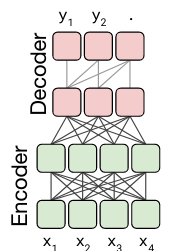
\includegraphics[scale=0.8]{figures/t5_architecture.png}
    \end{figure}
\end{frame}

\begin{frame}{Architecture of T5}
  \begin{itemize}
    \item Decoder is of similiar structure
    \item Includes a standard attention mechanism after each self-attention layer that attends to the output of the encode
    \item Self-attention mechanism: autoregressive or causal self-
    attention
    \item Output of the final decoder block is fed into a dense layer with a softmax output
    \item Attention mechanisms are split up into
    independent “heads” whose outputs are concatenated before being further processed.
    \item Relative position encoding is applied instead of sine based encoding
  \end{itemize}
\end{frame}

\begin{frame}{Pretraining of T5}
  \begin{itemize}
    \item T5 is pretrained in a parallel way using Cloud TPU pods
    \item T5 leveraged the Common Crawl dataset generated with web text
    \item Colossal Clean Crawled Corpus (C4) will be used
    \begin{itemize}
      \item Removed pages with less than 5 sentences 
      \item Removed any page containing a naughty word 
      \item Removed any lines with Javascript in it
      \item Removed any pages that contained "\{"
      \item Removed duplicate pages
    \end{itemize}
    \item C4 is roughly 750 GB with clean and natural text
    \item Realeased as part of the TensorFlow Datsets
  \end{itemize}
\end{frame}

\begin{frame}{Finetuning of T5}
    \begin{itemize}
      \item Finetuning on tasks from GLUE/SuperGLUE
      \begin{itemize}
        \item Question answering
        \item Sentence completion
        \item Natural language interference
      \end{itemize}
      \item Concatenating all GLUE/SuperGLUE datasets togheter
      \item Task have to be formatted in the same way
      \item A task specific prefix is added before feeding the text to the model:
      \item \texttt{translate English to German: <Text>}
    \end{itemize}
\end{frame}

\begin{frame}{Conclusion}
    \begin{itemize}
      \item Text-to-text based task formulation for generalizing Transformer architecture across language tasks works
      \item Model is still large and needs high computation power
      \item The field requires methods for stronger performance with cheaper models. Some work is performed on this through distillation, parameter sharing, and conditional computation
      \item  Formalizing task similarity can help us understand which unlabeled data must be used for a specific task
      \item Language-agnostic models can greatly boost the field, i.e. models that can be used regardless of language
    \end{itemize}
\end{frame}

\begin{frame}{Overview of T0~\cite{SanhWRBSACSLRDBXTSSKCNDCJWMSYPBWNRSSFFTBGBWR2021}}
    \begin{itemize}
      \item Training of T5 model on a subset of tasks and evaluating tasks the model was not trained on
      \item Does multitask prompted training improve generalization to unseen tasks?
      \item Does training on a wider range of prompts improve robustness to prompt wording?
      \item All datasets are given to the model in natural language prompted form to enable zero-shot experimentation
      \item Goal: Induce a model to better generalize to unseen tasks without requiring massive scale and being more robust to the
      wording choices of the prompts
    \end{itemize}
\end{frame}

\begin{frame}{Examples of zero-shot experimentation}
    \begin{figure}
        \center
        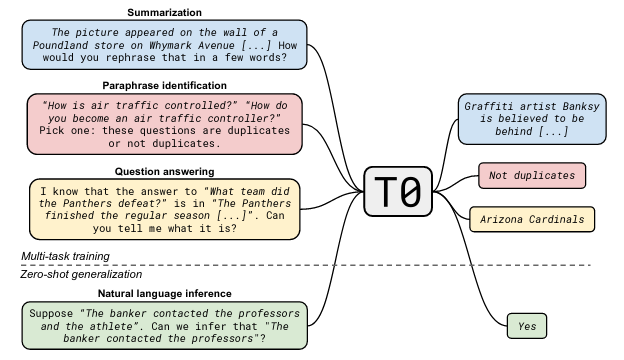
\includegraphics[scale=0.45]{figures/t0_examples.png}
    \end{figure}
\end{frame}

\begin{frame}{Examples of prompts}
    \begin{figure}
      \center
      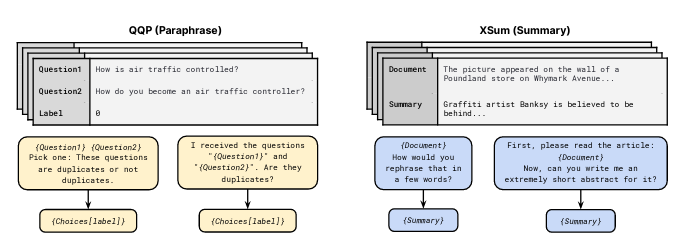
\includegraphics[scale=0.5]{figures/prompts.png}
    \end{figure}
\end{frame}

\begin{frame}{Datasets and tasks used to train}
  \begin{figure}
    \center
    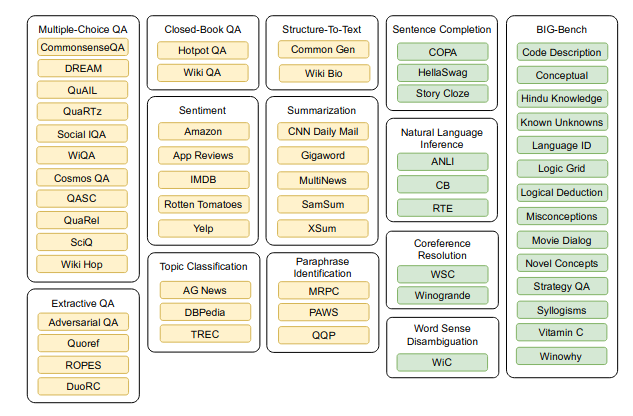
\includegraphics[scale=0.5]{figures/t0_datasets.png}
  \end{figure}
\end{frame}

\begin{frame}{Conclusion}
    \begin{itemize}
      \item Benefits of multitask training compared to only language modeling with an identical model and prompts
      \item T0 surpasses all GPT-3 models on 8 of 11 held-out datasets
      \item Model is 16 times smaller than GPT-3
      \item Model improves over a large baseline language model on 13 of 14 comparable tasks in the BIG-bench benchmark
      \item Training on more prompts per dataset consistently improves the median and decreases the variability of performance on held-out tasks
      \item Training on prompts from a wider range of datasets also generally improves the median but does not decrease the variability
    \end{itemize}
\end{frame}

\appendix
\section{\appendixname}

\bibliographyframe

\end{document}